\documentclass[a4paper,twocolumn]{article}
\usepackage[hmargin={1.1cm,1.1cm},vmargin={2.2cm,2cm}]{geometry}
%       includehead,     scale=0.85,centering,hoffset=-0.1cm,voffset=-0.5cm]{geometry} headheight=13.1pt ,portrait

%\usepackage[a4paper,portrait,twocolumn,includeheadfoot,
%            scale=0.85,centering,hoffset=-1cm]{geometry}
\usepackage[pdftex]{graphicx,color}
\usepackage{amsmath}
\usepackage{amssymb}
\usepackage{stmaryrd}
\usepackage[french]{babel}
\selectlanguage{french}
\usepackage{fancyhdr}
\usepackage{floatflt}
\usepackage{ucs}
\usepackage[utf8]{inputenc}
\usepackage[T1]{fontenc}
\usepackage[pdftex,colorlinks={true},urlcolor={blue},pdfauthor={remy Nicolai}]{hyperref}
\usepackage{makeidx}


%Options de hyperref pour les fichiers pdf g{\'e}n{\'e}r{\'e}s
%\hypersetup{pdfpagemode=None,colorlinks=true,pdffitwindow=true}
%\hypersetup{pdfpagemode=None,colorlinks=true}


%                 Chargement des symboles de l'AMS
%\input amssym
%pour que la compilation aille au bout
%\nofiles\scrollmode

%pr{\'e}sentation du compteur de niveau 2 dans les listes
\makeatletter
\renewcommand{\labelenumii}{\theenumii.}
\makeatother

%dimension des pages, en-t{\^e}te et bas de page
  %utilisation avec vmargin
   %\setpapersize{custom}{21cm}{29.7cm}
   %\setmarginsrb{1.5cm}{0cm}{3.5cm}{1cm}{15mm}{10mm}{0mm}{0mm}
%\setlength{\voffset}{-2cm}
%\setlength{\oddsidemargin}{-1cm}
%\setlength{\textheight}{25cm}
%\setlength{\textwidth}{17.3cm}
%\columnsep=5pt
% \columnseprule=0.5pt
%\columnseprule=0.5pt
%En tete et pied de page
\pagestyle{fancy}
\lhead{Lycée Hoche MPSI B}
%\rhead{}
%\rhead{25/11/05}
\lfoot{\tiny{Cette création est mise à disposition selon le Contrat\\ Paternité-Partage des Conditions Initiales à l'Identique 2.0 France\\ disponible en ligne http://creativecommons.org/licenses/by-sa/2.0/fr/
} }
\rfoot{\tiny{Rémy Nicolai \jobname pdf du \today}}

%\pagestyle{fancy}
%\lhead{MPSI B}
%\rhead{\today}
%\rfoot{\small{\jobname}}
\newcommand{\baseurl}{http://back.maquisdoc.net/data/}
\newcommand{\textesurl}{http://back.maquisdoc.net/data/devoirs_nicolair/}
\newcommand{\exosurl}{http://back.maquisdoc.net/data/exos_nicolair/}
\newcommand{\coursurl}{http://back.maquisdoc.net/data/cours_nicolair/}

\newcommand{\N}{\mathbb{N}}
\newcommand{\Z}{\mathbb{Z}}
\newcommand{\C}{\mathbb{C}}
\newcommand{\R}{\mathbb{R}}
\newcommand{\K}{\mathbf{K}}
\newcommand{\Q}{\mathbb{Q}}
\newcommand{\F}{\mathbf{F}}
\newcommand{\U}{\mathbb{U}}
\newcommand{\p}{\mathbb{P}}


\newcommand{\card}{\mathop{\mathrm{Card}}}
\newcommand{\Id}{\mathop{\mathrm{Id}}}
\newcommand{\Ker}{\mathop{\mathrm{Ker}}}
\newcommand{\Vect}{\mathop{\mathrm{Vect}}}
\newcommand{\cotg}{\mathop{\mathrm{cotan}}}
\newcommand{\cotan}{\mathop{\mathrm{cotan}}}
\newcommand{\sh}{\mathop{\mathrm{sh}}}
\newcommand{\ch}{\mathop{\mathrm{ch}}}
\newcommand{\argch}{\mathop{\mathrm{argch}}}
\newcommand{\argsh}{\mathop{\mathrm{argsh}}}
\newcommand{\tr}{\mathop{\mathrm{tr}}}
\newcommand{\rg}{\mathop{\mathrm{rg}}}
\newcommand{\rang}{\mathop{\mathrm{rg}}}
\newcommand{\val}{\mathop{\mathrm{val}}}

\newcommand{\Mat}{\mathop{\mathrm{Mat}}}
\newcommand{\MatB}[2]{\mathop{\mathrm{Mat}}_{\mathcal{#1}}\left( #2\right) }
\newcommand{\MatBB}[3]{\mathop{\mathrm{Mat}}_{\mathcal{#1} \mathcal{#2}}\left( #3\right) }

\renewcommand{\Re}{\mathop{\mathrm{Re}}}
\newcommand{\Ima}{\mathop{\mathrm{Im}}}
\renewcommand{\Im}{\mathop{\mathrm{Im}}}
\renewcommand{\th}{\mathop{\mathrm{th}}}
\newcommand{\repere}{$(O,\overrightarrow{i},\overrightarrow{j},\overrightarrow{k})$ }
\newcommand{\trans}{\mathstrut^t\!}
\newcommand{\cov}{\mathop{\mathrm{Cov}}}
\newcommand{\orth}[1]{#1^{\perp}}

\newcommand{\absolue}[1]{\left| #1 \right|}
\newcommand{\fonc}[5]{#1 : \begin{cases}#2 &\rightarrow #3 \\ #4 &\mapsto #5 \end{cases}}
\newcommand{\depar}[2]{\dfrac{\partial #1}{\partial #2}}
\newcommand{\norme}[1]{\left\| #1 \right\|}
\newcommand{\se}{\geq}
\newcommand{\ie}{\leq}
\newcommand{\serie}[1]{\left( \sum {#1}_n \right)_{n\in\N}}

\batchmode
 
\begin{document} 
\chead{ géométrie affine: énoncés.}
\begin{enumerate}
  \item \begin{tiny}(Ega01)\end{tiny} Rappel sur les conditions d'alignement ou de concours.
\begin{enumerate}
 \item Dans un plan muni d'un repère, on considère trois points $A_1$, $A_2$, $A_3$ respectivement de coordonnées $(x_1,y_1)$, $(x_2,y_2)$, $(x_3,y_3)$. Montrer que ces trois points sont alignés si et seulement si
\begin{displaymath}
 \begin{vmatrix}
  x_1 & y_1 & 1 \\
  x_2 & y_2 & 1 \\
  x_3 & y_3 & 1 \\
 \end{vmatrix}
=0
\end{displaymath}
\item Dans un plan, trois points non alignés $U$, $V$, $W$ sont fixés. On considère trois points $A_1$, $A_2$, $A_3$ respectivement barycentres de $U$, $V$, $W$ avec les coefficients $(x_1,y_1,z_1)$, $(x_2,y_2,z_2)$, $(x_3,y_3,z_3)$.
 Montrer que ces trois points sont alignés si et seulement si
\begin{displaymath}
 \begin{vmatrix}
  x_1 & y_1 & z_1 \\
  x_2 & y_2 & z_2 \\
  x_3 & y_3 & z_3 \\
 \end{vmatrix}
=0
\end{displaymath}
\item Les fonctions coordonnées $x$ et $y$ sont relatives à un repère fixé d'un plan. On considère trois droites d'équations
\begin{displaymath}
 \left\lbrace
\begin{aligned}
 ax+by+c &= 0\\a'x+b'y+c' &= 0\\a''x+b''y+c'' &= 0
\end{aligned}\right. 
\end{displaymath}
Montrer que ces droites sont parallèles ou concourantes si et seulement si
 \begin{displaymath}
  \begin{vmatrix}
   a&b&c\\a'&b'&c'\\a''&b''&c''
  \end{vmatrix}
=0
 \end{displaymath}

\end{enumerate} 
  \item \begin{tiny}(Ega02)\end{tiny} Dans un espace affine de dimension $n$, on considère une famille $(A_0,A_1,\cdots,A_n)$ de $n+1$ points qui ne sont contenus dans aucun hyperplan affine et une famille $(B_0,B_1,\cdots,B_n)$ de $n+1$ points quelconques. Montrer qu'il existe une unique application affine $f$ de l'espace dans lui même telle que  $f(A_i)=B_i$ pour tous les $i$ entre $0$ et $n$. 
  \item \begin{tiny}(Ega03)\end{tiny}
\begin{figure}[ht]
 \centering
 \input{Ega03_1.pdf_t}
 \caption{Exercice \arabic{enumi}}
 \label{fig:Ega03_1}
\end{figure}
Cet exercice propose deux parties indépendantes autour d'une même configuration.\newline
 Les points $A_1$, $A_2$, $A_3$ sont alignés sur une droite $\mathcal D$ dirigée par un vecteur $u$. Les points $A'_1$, $A'_2$, $A'_3$ sont alignés sur une droite $\mathcal D'$ dirigée par un vecteur $u'$. Tous ces points sont distincts du point d'intersection noté $O$ des deux droites. 
\begin{enumerate}
 \item Les points $B_1$, $B_2$, $B_3$ sont respectivement les intersections $(A_2,A'_3)\cap(A'_2,A_3)$, $(A_3,A'_1)\cap(A'_3,A_1)$, $(A_1,A'_2)\cap(A'_1,A_2)$ qui sont supposées non vides.\newline
Par des calculs de coordonnées dans le repère $(O,(u,v))$, montrer que les points $B_1$, $B_2$, $B_3$ sont alignés.\footnote{ce résultat est un cas particulier du théorème de l'hexagramme de Pascal. Les $B$ sont alignés lorsque les $6$ points $A_1,...$ sont sur une même conique. En utilisant Maple, cela peut se démontrer par le calcul. Les deux droites $\mathcal{D}$ et $\mathcal{D'}$ forment une conique dégénérée. (voir le problème \href{http://back.maquisdoc.net/data/devoirs_nicolair/AhexaP.pdf}{hexaP})}\\
On utilisera le résultat de l'exercice dt15 de la \href{\exosurl _fex_dt.pdf}{feuille sur les déterminants}. \`A savoir:
\begin{displaymath}
 \begin{vmatrix}
 \alpha_2'-\alpha_3' & \alpha_2 - \alpha_3 & \alpha_2\alpha_2'-\alpha_3\alpha_3' \\
 \alpha_3'-\alpha_1' & \alpha_3 - \alpha_1 & \alpha_3\alpha_3'-\alpha_1\alpha_1' \\
 \alpha_1'-\alpha_2' & \alpha_1 - \alpha_2 & \alpha_1\alpha_1'-\alpha_2\alpha_2'
\end{vmatrix}
=0
\end{displaymath}
pour des réels non nuls $\alpha_1$, $\alpha_2$, $\alpha_3$, $\alpha_1'$, $\alpha_2'$, $\alpha_3'$.
\item On définit trois applications affines $f_1$, $f_2$, $f_3$ par :
\begin{align*}
 \left\lbrace \begin{aligned}
  f_1(O)=&O\\ f_1(A_2)=&A_3 \\ f_1(A'_3)=&A'_2
 \end{aligned}\right. 
& &
\left\lbrace  \begin{aligned}
  f_2(O)=&O\\ f_2(A_3)=&A_1 \\ f_2(A'_1)=&A'_3
 \end{aligned}\right. 
& &
\left\lbrace  \begin{aligned}
  f_3(O)=&O\\ f_3(A_1)=&A_2 \\ f_3(A'_2)=&A'_1
 \end{aligned}\right. 
\end{align*}
Que peut-on dire de la matrice dans la base $(u,v)$ de la partie linéaire d'une de ces fonctions ? Montrer que ces fonctions commutent entre elles. Que vaut la composée des trois ?\newline
On suppose maintenant que 
\begin{displaymath}
 (A_1,A'_2)\parallel (A'_1,A_2)\text{ et } (A_2,A'_3)\parallel (A'_2,A_3)
\end{displaymath}
Que peut-on en déduire pour $f_3$ et $f_1$? Montrer que 
\begin{displaymath}
 (A_1,A'_3)\parallel (A'_1,A_3)
\end{displaymath}
(théorème de Pappus)
\end{enumerate}
 
  \item \begin{tiny}(Ega04)\end{tiny}
\begin{figure}[h!]
  \centering
  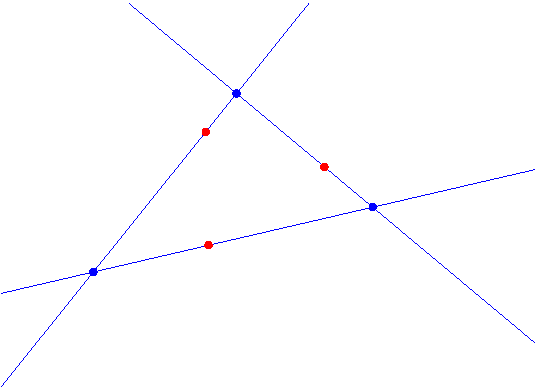
\includegraphics[width=7cm]{Ega04_1.pdf}
  % Egp11_1.pdf: 170x107 px, 72dpi, 6.00x3.77 cm, bb=0 0 170 107
  \caption{Exercice \arabic{enumi}: théorème de Ménéla{\"u}s.}
  \label{fig:Ega04_1}
\end{figure}

Les points $A$, $B$, $C$ d'un plan affine sont non alignés, les réels $\alpha$, $\beta$, $\gamma$ sont différents de $1$. Les points $L$, $M$, $N$ (voir figure \ref{fig:Ega04_1}) sont définis comme des barycentres de $A$, $B$, $C$ avec les coefficients suivants.
\begin{align*}
 L:(0,1,-\alpha) & & M:(-\beta, 0, 1) & & N:(1,-\gamma, 0)
\end{align*}
\begin{enumerate}
 \item Former une relation entre $\alpha$,$\beta$, $\gamma$ caractérisant l'alignement de $L$, $M$, $N$. Montrer que cette relation s'écrit
\begin{displaymath}
\frac{\overline{LB}}{\overline{LC}}\,
\frac{\overline{MC}}{\overline{MA}}\,
\frac{\overline{NA}}{\overline{NB}}=1 
\end{displaymath}
(théorème de Ménélaüs)
\footnote{voir la feuille \href{http://back.maquisdoc.net/data/temptex/fexgp.pdf}{Géométrie plane élémentaire}(exercices gp11.)}
\item Montrer que les droites $(A,L)$, $(B,M)$, $(C,N)$ sont concourantes ou alignées si et seulement si 
\begin{displaymath}
\frac{\overline{LB}}{\overline{LC}}\,
\frac{\overline{MC}}{\overline{MA}}\,
\frac{\overline{NA}}{\overline{NB}}=-1 
\end{displaymath}
(théorème de Céva)
\item Montrer que si $L$, $M$, $N$ sont alignés, les milieux des segments $AL$, $BM$, $CN$ sont alignés.\newline
On définit les points $L'$, $M'$, $N'$ comme des barycentres de $A$, $B$, $C$ avec les coefficients suivants.
\begin{align*}
 L':(0,-\alpha,1) & & M':(1, 0, -\beta) & & N':(-\gamma, 1, 0).
\end{align*}
Montrer que $L$, $M$, $N$ sont alignés si et seulement si $L'$, $M'$, $N'$ sont alignés. (les deux droites sont dites \emph{isotomiques})
\end{enumerate}
 
  \item \begin{tiny}(Ega05)\end{tiny} Cet exercice généralise ga04 en dimension $n$. Dans un espace affine de dimension $n$, on se donne $n+1$ points $A_1, A_2, \cdots, A_{n+1}$ qui ne sont pas dans un même hyperplan. On définit les points $B_1,\cdots,B_{n+1}$ par :
 \begin{align*}
  \forall i \in \{1,\cdots,n\} : \overrightarrow{B_iA_i} =& \lambda_i \overrightarrow{B_iA_{i+1}}\\
\overrightarrow{B_{n+1}A_{n+1}} =& \lambda_{n+1} \overrightarrow{B_nA_{1}}
 \end{align*}
Les $\lambda_i$ sont des réels différents de $0$ et de $1$.
\begin{enumerate}
\item Exprimer les points $B_i$ comme des barycentres de $A_1,\cdots,A_n$. En admettant que les points $B_i$ sont dans un même hyperplan si et seulement si le déterminant ($(n+1)\times(n+1)$) constitué par les coordonnées barycentriques est nul, montrer que les $B_i$ sont dans un même hyperplan si et seulement si
\begin{displaymath}
 \lambda_1\lambda_2\cdots \lambda_{n+1}=1
\end{displaymath}
\item On va retrouver le résultat précédent par une voie très différente.\newline
Montrer que le centre de la composée de plusieurs homothéties (lorsqu'il existe) est un barycentre des centres des homothéties qui interviennent dans la composition.\newline
Pour $i$ entre $1$ et $n+1$, on désigne par $h_i$ l'homothétie de centre $B_i$ et de rapport $\lambda_i$.\newline
Préciser $h_1\circ h_2\circ\cdots\circ h_{n+1}(A_1)$. Considérer de même $h_{n+1}\circ h_1\circ\cdots\circ h_{n}$ et ainsi de suite ... En déduire que si les $B_i$ sont dans un même hyperplan, le produit des $\lambda_i$ doit obligatoirement valoir $1$.
\end{enumerate}
 
  \item \begin{tiny}(Ega06)\end{tiny} Dans un plan, on se donne deux droites $\mathcal D_1$ et $\mathcal D_2$. Soit $a$ un réel strictement positif fixé. Pour tout point $M$, on note $M_1$ le symétrique de $M$ par rapport à $\mathcal D_1$ et $M_2$ le symétrique par rapport à $\mathcal D_2$.\newline
Déterminer l'ensemble des points $M$ tels que 
\begin{displaymath}
 M_1M_2 = a
\end{displaymath} 
  \item \begin{tiny}(Ega07)\end{tiny} Soit $u$ et $v$ des complexes fixés avec $|v|=1$. Montrer que la transformation du plan complexe 
\begin{displaymath}
 z\rightarrow u+ v\overline{z}
\end{displaymath}
est un antidéplacement. Montrer que c'est une réflexion si et seulement si $v=-\frac{u}{\overline{u}}$. 
  \item \begin{tiny}(Ega08)\end{tiny} Dans un $\R$-espace vectoriel $E$ de dimension $3$, on se donne un repère affine $(A,(i,j,k))$. Les fonctions coordonnées dans ce repère sont notées $x$, $y$, $z$.\newline
Soit $B$ le point de coordonnées $(1,1,1)$ dans ce repère. Soit $u$, $v$, $w$ trois vecteurs dont les coordonnées dans la base $(i,j,k)$ sont
\begin{displaymath}
u:(1,1,1),\hspace{0.3cm} v:(0,1,1),\hspace{0.3cm} w:(1,0,1)  
\end{displaymath}
Vérifier que $(B,(u,v,w))$ est un repère affine. On note $X$, $Y$, $Z$ les fonctions coordonnées dans ce repère. Exprimer $x$, $y$, $z$ en fonction de $X$, $Y$, $Z$ puis $X$, $Y$, $Z$ en fonction de $x$, $y$, $z$. 
  \item \begin{tiny}(Ega09)\end{tiny} Dans un $\R$-espace vectoriel $E$ de dimension $3$, on se donne un repère affine $(A,(i,j,k))$. Les fonctions coordonnées dans ce repère sont notées $x$, $y$, $z$.\newline
On considère trois fonctions $X$, $Y$, $Z$
\begin{displaymath}
\left\lbrace 
\begin{aligned}
  X &= x+y+1 \\ Y &= y + z \\ Z &= x + z - 1
\end{aligned}
\right. 
\end{displaymath}
Déterminer un repère affine $(B,(u,v,w))$ tel que les fonctions coordonnées dans ce repère soient $X$, $Y$, $Z$.
 
  \item \begin{tiny}(Ega10)\end{tiny} Soit $E$ un $\R$-espace vectoriel de dimension $2$. On rappelle que l'ensemble des fonctions de $E$ dans $\R$ est un $\R$-espace vectoriel noté $\mathcal{F}(E,\R)$. L'ensemble $E^*$ des formes linéaires est un sous-espace vectoriel de $\mathcal{F}(E,\R)$. Pour tout $\lambda\in \R$, on note $\overline{\lambda}$ la fonction constante de valeur $\lambda$ de $E$ dans $\R$. On note ici $\overline{\R}$ l'ensemble des fonctions constantes de $\mathcal{F}(E,\R)$. Il est évident que $\overline{\R}$ est un sous-espace vectoriel de $\mathcal{F}(E,\R)$. On note
\begin{displaymath}
  F = E^* + \overline{\R}
\end{displaymath}
Un élément de $F$ sera appelé \emph{fonction numérique affine}.
\begin{enumerate}
  \item Montrer que $E^*$ et $\overline{\R}$ sont supplémentaires dans $F$. En déduire une base de $F$. Toute fonction numérique affine se décompose donc de manière unique comme la somme d'une \emph{partie linéaire} et d'une \emph{partie constante}.
  \item Soit $\varphi \in F$, discuter de la nature de $D_\varphi = \varphi^{-1}(\{0\})$ (image réciproque du singleton).
  \item Soit $\varphi_1$, $\varphi_2$, $\varphi_3$ des fonctions numériques affines non constantes. Discuter suivant $\rg(\varphi_1,\varphi_2,\varphi_3)$ de la configuration géométrique de $D_{\varphi_1}$, $D_{\varphi_2}$, $D_{\varphi_3}$.
\end{enumerate}
 
\end{enumerate} 
\clearpage 
\chead{géométrie affine: corrigés.}
\begin{enumerate}
  \item Cga01.tex manque. 
  \item Cga02.tex manque. 
  \item Cga03.tex manque. 
  \item \begin{tiny}(Cga04)\end{tiny}
\begin{enumerate}
  \item D'après l'expression barycentrique de la condition d'alignement, les points $L$, $M$, $N$ sont alignés si et seulement si
\begin{displaymath}
  \begin{vmatrix}
    0      & 1       & -\alpha \\
    -\beta & 0       & 1       \\
    1      & -\gamma & 0
  \end{vmatrix}
=0.
\end{displaymath}
Ce déterminant est égal à $1 - \alpha \beta \gamma$.\newline
En projetant sur un vecteur unitaire de la droite $(BC)$, on passe de la définition du barycentre à une expression de $\alpha$ comme quotient de valeurs algébriques:
\begin{displaymath}
  \overrightarrow{LB} - \alpha \overrightarrow{LC}= \overrightarrow{0}
  \Rightarrow
  \overline{LB} - \alpha \overline{LC}= 0.
\end{displaymath}
On en déduit la condition demandée.

  \item On utilise cette fois la condition de concours de trois droites exprimée comme la nullité d'un déterminant formé à partir des équations des droites. On forme les équations des droites dans le repère $(A,\overrightarrow{AB},\overrightarrow{AC})$:
\begin{align*}
  (AL) &:& \alpha x + y = 0 \\
  (BM) &:& x + (1-\beta)y - 1 = 0 \\
  (CN) &:& (1-\gamma)x - \gamma y + \gamma = 0
\end{align*}
La condition demandée (théorème de Ceva) vient du calcul du déterminant
\begin{displaymath}
  \begin{vmatrix}
    \alpha   & 1       & 0 \\
    1        & 1-\beta & -1 \\
    1-\gamma & -\gamma & \gamma 
  \end{vmatrix}
  =
  \begin{vmatrix}
    \alpha   & 1       & 0 \\
    0        & -\beta & -1 \\
    1        & 0      & \gamma 
  \end{vmatrix}
\end{displaymath}
en enlevant la troisième colonne aux deux premières.
\begin{displaymath}
  = - 1 - \alpha \beta \gamma.
\end{displaymath}

  \item Considérons
\begin{displaymath}
  \sin (\widehat{NB})\, \overrightarrow{OA} - \sin (\widehat{NA})\, \overrightarrow{OB}.
\end{displaymath}
Sa projection sur la direction orthogonale à $\overrightarrow{ON}$ est
\begin{displaymath}
  \sin (\widehat{NB})\, \sin (\widehat{NA}) - \sin (\widehat{NA})\, \sin (\widehat{NB})=0.
\end{displaymath}
Il est donc de même direction que $\overrightarrow{ON}$.\newline
Remarquons que sa projection sur $\overrightarrow{ON}$ est
\begin{multline*}
  \sin (\widehat{NB})\, \cos (\widehat{NA}) - \sin (\widehat{NA})\, \cos (\widehat{NB})\\
  = \sin \left( \widehat{NB} - \widehat{NA}\right).
\end{multline*}
Elle est nulle si et seulement si $A$ et $B$ sont diamétralement opposés.\newline
On peut former des vecteurs analogues pour $M$ et $L$. Les points $M$, $N$, $L$ sont sur un même grand cercle si et seulement si les vecteurs sont dans un même plan. Cela se traduit par la nullité du déterminant formé par les coordonnées dans la base $\left( \overrightarrow{OA}, \,\overrightarrow{OB}, \,\overrightarrow{OC}\right)$
\begin{displaymath}
  \begin{vmatrix}
    0                          & \sin(\overrightarrow{MC})  & \sin(\overrightarrow{NB}) \\ 
    \sin(\overrightarrow{LC})  & 0                          & -\sin(\overrightarrow{NA})  \\
    -\sin(\overrightarrow{LB}) & -\sin(\overrightarrow{MA}) & 0 
  \end{vmatrix}
.
\end{displaymath}
Ce déterminant se traite comme dans la question a.

  \item Pour caractériser l'alignement des milieux, on utilise encore la condition avec les coordonnées barycentriques. Il faut faire attention à prendre la même masse pour obtenir les coordonnées barycentriques d'un milieu. Par exemple, les coordonnées du milieu de $AL$ sont
\begin{displaymath}
  A (1-\alpha,0,0) + L(0,1,-\alpha) \rightarrow (1-\alpha, 1, -\alpha)
\end{displaymath}
De même pour les autres points. On conclut avec un calcul de déterminant
\begin{displaymath}
\begin{vmatrix}
  1- \alpha & 1       & -\alpha \\
  -\beta    & 1-\beta & 1 \\
  1         & -\gamma & 1-\gamma
\end{vmatrix}
= \cdots = 2(1-\alpha \beta \gamma).
\end{displaymath}

Chaque condition d'alignement se traduit par la nullité d'un déterminant
\begin{align*}
  L, M, N \text{ alignés } &\Leftrightarrow D = 0 \\
  L', M', N' \text{ alignés } &\Leftrightarrow  D' = 0
\end{align*}
avec
\begin{displaymath}
  D = 
\begin{vmatrix}
  0      & 1       & - \alpha \\
  -\beta & 0       & 1 \\
  1      & -\gamma & 0
\end{vmatrix}
\end{displaymath}
\begin{displaymath}
  D' = 
\begin{vmatrix}
  0       & - \alpha & 1  \\
  1       & 0       & -\beta \\
  -\gamma & 1 & 0
\end{vmatrix}
\end{displaymath}
En développant, on trouve 
\begin{displaymath}
  D = D' = 1 - \alpha \beta \gamma
\end{displaymath}
ce qui assure l'équivalence des alignements.
\end{enumerate}
 
  \item Cga05.tex manque. 
  \item Cga06.tex manque. 
  \item Cga07.tex manque. 
  \item Cga08.tex manque. 
  \item Cga09.tex manque. 
  \item Cga10.tex manque. 
\end{enumerate} 
\end{document}